\documentclass[11pt,a4paper]{article}

% ---------- Idioma y codificación ----------
\usepackage[T1]{fontenc}
\usepackage[utf8]{inputenc}
\usepackage[spanish,es-tabla,es-nodecimaldot]{babel}
\usepackage{lmodern}
\usepackage{textcomp}
\usepackage{csquotes}

% ---------- Página ----------
\usepackage[a4paper,margin=3cm]{geometry}
\usepackage{setspace}
\onehalfspacing

% ---------- Matemática, tablas y figuras ----------
\usepackage{amsmath,amssymb,bm}
\usepackage{booktabs}
\usepackage{graphicx}
\usepackage{float}
\usepackage[labelfont=bf,labelsep=period,justification=raggedright,singlelinecheck=false,skip=6pt]{caption}
\captionsetup[figure]{name=Gráfico}
% Ubicación de tablas y gráficos del anexo: permite llenar mejor cada página
\renewcommand{\topfraction}{0.9}\renewcommand{\bottomfraction}{0.8}\renewcommand{\textfraction}{0.05}
\renewcommand{\floatpagefraction}{0.75}\setcounter{topnumber}{3}\setcounter{bottomnumber}{3}\setcounter{totalnumber}{5}
\makeatletter\setlength{\@fptop}{0pt}\makeatother

% ---------- Bibliografía (APA 7) ----------
\usepackage[style=apa,backend=biber]{biblatex}
\addbibresource{referencias.bib}

\usepackage{xurl}
\usepackage[hidelinks]{hyperref}

\title{¿Existe pass-through de los impuestos municipales a los precios? Evidencia para el caso de Lanús}
\author{Kevin Pagnotta}
\date{Noviembre de 2026\\[1.5ex]\footnotesize Documento bajo licencia \href{https://creativecommons.org/licenses/by-nc-nd/4.0/deed.es}{CC BY-NC-ND 4.0}. Código de replicación: \url{https://github.com/kevinlpagnotta/precios-sepa}}

\begin{document}
\maketitle


\section{Introducción}

En diciembre de 2023 Argentina transitó un cambio de gobierno. Javier Milei, representante del partido de La Libertad Avanza, asumió el mandato luego de ganar el balotaje a Sergio Massa, candidato a presidente del partido oficialista que gobernó el país entre 2020-23. La situación macroeconómica era endeble y requería de una serie de correcciones. Puntualmente, el ejecutivo naciente heredó un déficit fiscal que representó el 6\% del PIB a finales de 2023. Esto motivó un fuerte ajuste fiscal, que llevó al país a alcanzar dos años consecutivos de superávit fiscal primario por primera vez desde el año 2008, algo poco habitual para los estándares locales.

El ordenamiento de las cuentas públicas se llevó adelante mediante un fuerte ajuste del gasto público, que pasó de representar el 20\% del PIB a la zona del 15\% del PIB entre 2023 y el período 2024-25. Buena parte de este recorte del gasto recayó en las transferencias no automáticas que realiza el Sector Público Nacional a las provincias, las cuales pasaron de representar el 0,8\% del PIB al 0,2\% del PIB entre el 2023 y el 2024. La merma de los recursos nacionales a provincias generó que los distritos al interior de cada una de ellas vean reducir los ingresos transferidos, tanto por la jurisdicción de pertenencia como aquellos programas que eran directamente ofrecido por el Sector Público Nacional.

Como respuesta a un contexto más adverso, una serie de municipalidades comenzaron a elevar los diferentes impuestos que cobran a las empresas por operar en el distrito. Un caso testigo de esto fue Lanús. En abril del 2024, la municipalidad mediante la Ordenanza N° 13.772 modificó el cuadro tarifario y el código de actividad de empresas que operan en el sector del comercio. Los establecimientos fueron divididos en tres grandes grupos: 1) Venta al por menor en minimercados (471130); 2) Venta al por menor en supermercados (471120); y 3) Venta al por menor en hipermercados (471110). Con este nuevo cuadro por actividad, la Tasa por Inspección de Seguridad e Higiene (TSH) se modificó, pasando de una carga plana del 2,3\% (2\% TSH y 0,3\% que provenía de otros cargos como ambientales) a un cómputo diferenciado por tipo de actividad. Ahora, la TSH para minimercados se redujo al 1\%, la de supermercados es del 2\% y la de hipermercados pasó al 6\%. Es decir, una elevación de 3,7 p.p. para las cadenas que operan con grandes superficies.

El 1 de agosto de 2024, el Decreto municipal N° 2.296 estableció que el nuevo nomenclador de actividades y sus alícuotas comenzarían a regir sobre la facturación de agosto de 2024, manteniendo el calendario de vencimientos vigente. El nuevo esquema se publicó en el Boletín Oficial municipal el 16 de septiembre de 2024 y, el 19 de septiembre, el Decreto N° 2.837 abrió los códigos de actividad con sus respectivas alícuotas y prorrogó al 27 de septiembre el vencimiento de la declaración jurada, el primero liquidado con la nueva alícuota a partir de agosto. Las cadenas que operan en grandes superficies respondieron de inmediato y anunciaron un traslado directo a los precios de góndola\footnote{\url{https://www.infobae.com/economia/2024/09/16/los-supermercados-en-pie-de-guerra-por-las-tasas-municipales-aumentaron-33-los-precios-en-lanus/}}.

En el presente documento, se extiende lo expuesto en el artículo web \href{https://kevinlpagnotta.github.io/precios-sepa/}{\enquote{Busque, compare y después compre: los precios en el AMBA}} con una mayor rigurosidad técnica. Tomando la base de Precios Claros (SEPA) con precios por cadena ubicado a nivel territorial, se evaluará mediante diferencias en diferencias y event study si el aumento de las tasas efectivamente se tradujo en un aumento de los precios y si fue sostenido en el tiempo. En este sentido, el artículo se estructura de la siguiente manera. Luego de la Introducción, la sección 2 abordará un repaso de la literatura, exhibiendo resultados ante medidas similares en otros países. En la sección 3 se presenta la estrategia empírica y los resultados y las verificaciones de robustez podrán verse en la sección 4 y 5, respectivamente. Por último, se presentará una conclusión final en la sección 6.

\section{Antecedentes}

La estructura de mercados regionales y acotados por límites jurisdiccionales viene ganando espacio en la literatura reciente. Esto se debe a que una empresa con presencia nacional se enfrenta a una serie de diferencias en las jurisdicciones que operan. La estructura del mercado puede variar a través de las diferentes jurisdicciones. El nivel de ingreso, los gustos y preferencias de una persona que vive en Buenos Aires no tiene por qué ser la misma de aquella que vive en Córdoba, e incluso al interior de cada una de las provincias existen diferencias en la demanda de los individuos. Del mismo modo, las empresas que operan al interior de cada provincia se enfrentan a diferentes condiciones. Pueden tener una presencia territorial más o menos monopólica, y se enfrentan a regulaciones, impuestos y salarios diferentes.

No obstante, las heterogeneidades sectoriales pueden verse supeditadas a políticas de pricing centralizadas según la política de las diferentes empresas. Esta centralidad en las decisiones puede conducir a precios uniformes al interior de las cadenas \parencite{dellavigna2019}, derivando en precios homogéneos y subóptimos entre las diferentes jurisdicciones al interior de una cadena. De hecho, viendo el total del AMBA (Ciudad Autónoma de Buenos Aires + 23 principales partidos del conurbano) expuesto en la Tabla~\ref{tab:dispersion} (véase Anexo I) se observa este comportamiento. Los precios idénticos (con una diferencia de \(\pm\)0,25\%) alcanzan el 84\% para octubre del 2026 entre los distintos partidos, y al mirar dentro de un mismo partido para aquellas cadenas que tengan un formato con más de dos sucursales crece hasta el 90\%. Incluso en situaciones de aceleración del nivel general de precios (como en diciembre del 2023 cuando la tasa de inflación se aceleró al 25,5\% mensual en Argentina), fenómeno asociado a una mayor dispersión, los precios idénticos se mantienen razonablemente elevados (69\% entre distintos partidos y 77\% mismo partido), algo consistente con la evidencia hallada por diferentes autores \parencite{nakamura2008,aparicio2021,hitsch2021}.

Sin embargo, la regularidad registrada en la uniformidad de precios de las distintas cadenas no significa que las empresas no actúen ante shocks locales. En concreto, medidas tomadas en jurisdicciones específicas que afecten la estructura de costos de las empresas pueden trasladarse a los precios de venta, generando por consiguiente una mayor diferenciación de precio al interior de las cadenas. De hecho, \textcite{butters2022} examinan 68 cambios de impuestos específicos y 76 impuestos a la venta a nivel local que afectan a productos como la cerveza, el licor, cigarrillos y sodas, y encuentran que los shocks locales son pasados a los precios por parte de las cadenas para una jurisdicción delimitada, sin generar spillovers para el resto de las cadenas ubicadas en otra locación. Asimismo, una vasta literatura encuentra evidencia de pass-through del aumento de impuestos a bebidas azucaradas en Filadelfia y Boulder \parencite{cawley2018,roberto2019,seiler2020}, con un traspaso a precios que oscila entre el 50\% y el 100\%, dependiendo del comercio (supermercado, farmacia, restaurante) y del tipo de relevamiento (online, relevamiento en campo). Asimismo, se encuentra evidencia de que la venta de bebidas azucaradas se reduce, pero la magnitud es menos de la mitad cuando se evalúa las consecuencias sobre otras localidades fuera de la ciudad que ve crecer sus ventas en este tipo de bebidas.

\section{Datos y estrategia empírica}

La base de datos del estudio es Precios Claros-SEPA, que es provista por la Secretaría de Industria y Comercio y la cual contiene información diaria de precios de venta de las diferentes grandes empresas minoristas que operan a nivel nacional. El presente trabajo se limita a los datos correspondientes a la Provincia de Buenos Aires y la Ciudad Autónoma de Buenos Aires. La base consiste en tres archivos, compuesto por la llave comercio (código de id por razón social, banderas, cuit y nombres), llaves sucursales (latitud, longitud, identificador de sucursal, código postal, entre otros) y productos (id de comercio, bandera, sucursal, código EAN, producto, descripción, marca, precio de lista, etc.).

Para el presente estudio, se cuenta con la serie desde junio del 2021 a octubre de 2026, lo que permite utilizar una ventana amplia para evaluar el impacto de la TSH de Lanús tomando desde abril del 2024 a octubre del 2025. Esto no está exento de dificultades propias de la base, con períodos de reporte vacío, fluctuaciones en el reporte de EAN e integración permanente de nuevas banderas/EAN desde junio del 2025. Precisamente, no se cuenta con datos disponibles para ChangoMás entre septiembre y noviembre del 2024, justo en el momento en el que se produce el aumento del impuesto. No obstante, se tiene información para Coto y Vea (Cencosud), lo que permite llevar adelante el análisis.

\subsection{Diferencias en diferencias}

La estrategia empírica compara el precio de un mismo producto, vendido en el mismo formato/bandera de local (se compara Carrefour Express con Carrefour Express, Cencosud Vea con Cencosud Vea, etc.), entre Lanús y el resto del AMBA, antes y después del aumento de la TSH. La unidad de observación es el producto \(i\) (código EAN), en el formato \(f\), en el partido \(p\) y en el mes \(t\). El precio \(P_{ifpt}\) es el promedio mensual de los precios de lista informados a SEPA por las sucursales de ese formato en el partido, y la variable dependiente es su logaritmo multiplicado por cien:

\begin{equation}\label{eq:1}
  y_{ifpt} = 100 \cdot \ln P_{ifpt}
\end{equation}

de modo que las diferencias en \(y\) se leen, aproximadamente, como diferencias porcentuales de precios.

El grupo tratado son los hipermercados de Lanús alcanzados por la alícuota de 6\% (código 471110): Coto y Vea. ChangoMás queda excluido por lo mencionado más arriba. El grupo de control son los mismos formatos en los demás partidos del AMBA donde operan: 20 partidos en el caso de Coto y 7 en el de Vea, que no tiene locales en los partidos vecinos a Lanús. Comparar cada formato consigo mismo evita que el resultado dependa de diferencias de skus informados o de nivel de precios entre banderas de una misma empresa.

La muestra es un panel balanceado por formato: se conservan solo los productos con precio en todos los meses de la ventana (abril de 2024 a octubre de 2025) y en todos los partidos donde opera el formato. Así, la comparación se hace siempre sobre la misma canasta y los cambios en la cobertura de SEPA no alteran los resultados. El panel reúne 2.517 productos de Coto en 21 partidos y 601 productos de Vea en 8 partidos.

La especificación principal es la siguiente:

\begin{equation}\label{eq:2}
  y_{ifpt} = \delta\left( \text{Lanús}_{p} \times \text{Post}_{t} \right) + \alpha_{ifp} + \lambda_{ift} + \varepsilon_{ifpt}
\end{equation}

donde \(\text{Lanús}_{p}\) vale uno para los locales de Lanús y \(\text{Post}_{t}\) vale uno a partir de octubre de 2024. El efecto fijo \(\alpha_{ifp}\) absorbe las diferencias permanentes de nivel del precio de cada producto en cada partido, y el efecto fijo \(\lambda_{ift}\) absorbe todo lo que es común a un producto, en un formato y un mes, en todo el AMBA. En consecuencia, \(\delta\) se identifica únicamente a partir de la variación del precio del mismo producto en Lanús respecto del resto del AMBA, en el mismo mes:

\begin{equation}\label{eq:3}
  \delta = \left( {\bar{y}}_{\text{post}}^{\,\text{Lanús}} - {\bar{y}}_{\text{pre}}^{\,\text{Lanús}} \right) - \left( {\bar{y}}_{\text{post}}^{\,\text{resto}} - {\bar{y}}_{\text{pre}}^{\,\text{resto}} \right)
\end{equation}

El supuesto de identificación es el de tendencias paralelas: en ausencia del aumento de la tasa, la diferencia de precios entre Lanús y el resto del AMBA para un mismo producto y formato se habría mantenido constante. Como especificación alternativa, y siguiendo a \textcite{cawley2018}, se estima también una versión con efectos fijos aditivos, que reemplaza \(\lambda_{ift}\) por un efecto fijo de mes \(\mu_{t}\) común a todos los productos.

En cuanto al mes de referencia, el Decreto N° 2.296 dispuso que la nueva alícuota se aplicara a la facturación de agosto de 2024. Julio de 2024 es, por lo tanto, el último mes en que los hipermercados tributaron con la alícuota anterior, y se toma como referencia. Agosto y septiembre de 2024 se excluyen de la estimación por tratarse de meses de transición: en agosto la nueva alícuota ya se aplicaba sobre la facturación, pero la norma todavía no se había publicado en el Boletín Oficial (16 de septiembre de 2024), y el precio promedio de septiembre mezcla días anteriores y posteriores a esa publicación. Además, el primer pago con la nueva alícuota venció el 27 de septiembre de 2024, luego de que el Decreto N° 2.837 abriera los códigos de actividad y prorrogara ese vencimiento. El período posterior comienza en octubre de 2024. Los errores estándar se agrupan por producto, lo que permite que los shocks de un mismo producto estén correlacionados entre meses y partidos.

Por último, la magnitud de \(\delta\) puede compararse con la que correspondería a un traslado completo de la tasa. La tasa grava la facturación neta de IVA: si \(P\) es el precio de góndola, \(v\) la alícuota de IVA y \(\tau\) la alícuota de la tasa, el ingreso neto por unidad que retiene el comercio es

\begin{equation}\label{eq:4}
  R = \frac{P}{1 + v}(1 - \tau)
\end{equation}

Si el comercio traslada la totalidad del aumento, de modo que su ingreso neto por unidad no cambia cuando la alícuota pasa de \(\tau_{0} = 0{,}023\) a \(\tau_{1} = 0{,}06\), el precio debe aumentar en

\begin{equation}\label{eq:5}
  100 \cdot \ln\frac{P_{1}}{P_{0}} = 100 \cdot \ln\frac{1 - \tau_{0}}{1 - \tau_{1}} = 100 \cdot \ln\frac{0{,}977}{0{,}94} \approx 3{,}86
\end{equation}

El IVA se cancela en el cociente, por lo que no afecta el cálculo. La tasa de traslado se define entonces como \(\theta = \widehat{\delta}/3{,}86\): un valor de 100\% indica que el aumento de la tasa se trasladó por completo a los precios.

\subsection{Estudio de eventos (\textit{event study})}

La estimación de la ecuación~\eqref{eq:2} resume el efecto en un único coeficiente, pero no muestra cómo evolucionó la diferencia de precios mes a mes. Para ello se estima un estudio de eventos (event study), que reemplaza el término \(\text{Lanús}_{p} \times \text{Post}_{t}\) por una interacción de Lanús con cada mes de la ventana:

\begin{equation}\label{eq:6}
  y_{ifpt} = \sum_{k \neq \text{jul-24}}\delta_{k}\left( \text{Lanús}_{p} \times \mathbf{1}\lbrack t = k\rbrack \right) + \alpha_{ifp} + \lambda_{ift} + \varepsilon_{ifpt}
\end{equation}

con los mismos efectos fijos y el mismo agrupamiento de errores que la especificación principal. Cada coeficiente \(\delta_{k}\) mide la diferencia de precios entre Lanús y el resto del AMBA en el mes \(k\), en relación con la diferencia en julio de 2024, que se normaliza a cero.

El estudio de eventos cumple dos funciones. La primera es evaluar el supuesto de tendencias paralelas: si la diferencia entre Lanús y el resto del AMBA era estable antes del aumento, los coeficientes de abril a junio de 2024 deberían ser cercanos a cero. Agosto de 2024 merece una mención aparte: la nueva alícuota ya se aplicaba sobre la facturación de ese mes, pero la norma todavía no se había publicado, por lo que un coeficiente cercano a cero indicaría que las cadenas no ajustaron sus precios antes de la publicación. La segunda es describir la dinámica del efecto: cuándo se produce el salto de precios y si se mantiene en el tiempo o se revierte en los meses siguientes.

\section{Resultados}

Siguiendo al Gráfico~\ref{fig:tendencias} (Anexo I) se observa la evolución del precio promedio expresado en logaritmos para una misma canasta de Lanús y el resto del AMBA. Allí se puede observar cómo ambas series evolucionan de forma superpuestas hasta agosto del 2024, tanto para los comercios de hipermercados y supermercados. No obstante, a partir de septiembre de 2024, la tendencia de Lanús sufre un quiebre y se despega para hipermercados (sector alcanzado a la nueva tasa del 6\%), manteniendo una tendencia paralela, pero de mayor nivel luego de un año de la aplicación del aumento de la tasa. Contrastando con esto, se nota cómo la evolución de los supermercados (DIA y Carrefour Express) mantienen inalterada la evolución de precios, superponiéndose durante el mismo lapso temporal.

Asimismo, la Tabla~\ref{tab:did} muestra los resultados para las estimaciones de la ecuación~\eqref{eq:2}. La especificación principal (columna 2) resulta en un aumento del 3,22\% para los hipermercados de Lanús (error estándar de 0,05) respecto a los mismos productos del resto del AMBA. Con la especificación de efectos fijos aditivos sugerida por \textcite{cawley2018} el efecto es aún mayor (3,52\%). Además, se nota una discrepancia en la política de traslado por cadenas: el efecto hallado para Coto es del 3,42\% y el de Vea del 2,30\%.

Evaluando el traslado (pass-through), el efecto estimado equivale al 83\% del aumento de precios que correspondería a un traslado completo de la tasa (3,86\%), con 89\% en Coto y 59\% en Vea. El resultado es consistente con lo anunciado por las cadenas y con los reportes de la literatura empírica, con un rango que varía entre el 50\% y el 100\%. Dicho eso, el menor traslado estimado para Vea debe leerse con cautela: la muestra es más chica (601 productos) y la comparación descansa en solo 7 partidos de control.

Por último, los resultados del estudio de eventos muestran que la respuesta de las cadenas se mantuvo en el tiempo y que no hay signos de reversión. La Tabla~\ref{tab:es} y el Gráfico~\ref{fig:es} del Anexo I presentan los coeficientes: hasta agosto de 2024 son cercanos a cero, en septiembre se produce un salto a 1,49 y, desde octubre, se mantienen en torno a 3 hasta un año después de la aplicación de la medida.

\section{Verificación de validez y robustez}

Con un único partido tratado, los errores estándar agrupados pueden subestimar la incertidumbre de la estimación: la variación que identifica \(\delta\) proviene de una sola jurisdicción, y los métodos de inferencia habituales suponen un número grande de grupos tratados \parencite{conley2011,ferman2019}. Por eso, como inferencia de referencia se utiliza una prueba de permutación entre partidos, en la línea de \textcite{conley2011} y de \textcite{abadie2010}.

El procedimiento consiste en excluir a Lanús de la muestra y asignar el tratamiento, de a uno por vez, a cada uno de los \(Q\) partidos de control. Para cada partido \(q\) se define \(D_{pt}^{(q)} = \mathbf{1}\lbrack p = q\rbrack \times \text{Post}_{t}\) y se reestima la ecuación~\eqref{eq:2}, lo que da un efecto placebo \({\widehat{\delta}}^{(q)}\). Si el aumento de la tasa no tuvo efecto, el coeficiente de Lanús debería ser uno más de esa distribución. El p-valor de permutación es la proporción de partidos, incluido Lanús, cuyo efecto es al menos tan grande como el de Lanús en valor absoluto:

\begin{equation}\label{eq:7}
  p = \frac{1}{Q + 1}\sum_{q = 1}^{Q + 1}\mathbf{1}\left\lbrack \left| {\widehat{\delta}}^{(q)} \right| \geq \left| {\widehat{\delta}}_{\text{Lanús}} \right| \right\rbrack
\end{equation}

Como el p-valor depende de la cantidad de partidos, su valor mínimo posible es \(1/(Q + 1)\): 0,048 con los 21 partidos de Coto y 0,125 con los 8 partidos de Vea.

El Gráfico~\ref{fig:perm} (Anexo I) muestra el resultado. Al asignar el tratamiento a cada uno de los otros 20 partidos, los efectos placebo se ubican entre \textminus{}0,18\% y 0,36\%, mientras que el efecto en Lanús es de 3,22\%. Ningún partido se acerca a Lanús, por lo que el p-valor es de 0,048, el mínimo posible con 21 partidos. Lo mismo ocurre en Coto (p = 0,048). En Vea el p-valor es de 0,125, que también es el mínimo posible con 8 partidos: Lanús tiene el mayor efecto entre los partidos donde opera Vea, pero con tan pocos partidos la prueba no puede alcanzar los niveles de significatividad convencionales.

La misma lógica se aplica al estudio de eventos. La franja gris del Gráfico~\ref{fig:es} muestra, para cada mes, el rango de coeficientes que se obtiene al asignar el tratamiento a cada uno de los demás partidos. Los coeficientes de Lanús previos al aumento son cercanos a cero (entre \textminus{}0,10 y 0,04) y caen dentro de esa franja, por lo que las series de precios de Lanús y del resto del AMBA evolucionaban de forma superpuesta antes de la suba de la tasa. Los coeficientes posteriores, en cambio, se ubican muy por encima del rango de los demás partidos.

Por último, se realiza una prueba placebo con locales de Lanús que no quedaron alcanzados por el aumento: los supermercados (DIA y Carrefour Express), cuya alícuota no aumentó (de hecho, se redujo levemente). Se estima la ecuación~\eqref{eq:2} para estos formatos, comparándolos con los mismos formatos en el resto del AMBA. Si el salto de precios observado en los hipermercados reflejara un shock propio de Lanús (por ejemplo, un cambio en la demanda o en los costos de operar en el partido), también debería observarse en estos locales.

La Tabla~\ref{tab:placebo} y el Gráfico~\ref{fig:es_placebo} (Anexo I) muestran que no es así. El efecto estimado para los supermercados es de \textminus{}0,02\% (error estándar de 0,01), con un p-valor de permutación de 0,667, y es igualmente nulo para cada cadena por separado. Los coeficientes del estudio de eventos se mantienen en torno a cero durante toda la ventana. En conjunto, la ausencia de diferencias previas al aumento, la magnitud del efecto en relación con los demás partidos y la ausencia de efecto en los supermercados indican que el aumento de precios de los hipermercados de Lanús se explica por el aumento de la tasa.

\section{Conclusiones}

La estrategia de pricing de las grandes cadenas que operan en el AMBA replica los comportamientos registrados en otros países. Esto se traduce en precios marcadamente distintos entre cadenas, pero una política de precios en gran medida uniforme al interior de cada una de ellas. Como consecuencia, los precios al interior del AMBA son relativamente homogéneos y poco sensibles a la estructura de mercado de cada una de las jurisdicciones. No obstante, en línea con la evidencia internacional, las cadenas responden ante la emergencia de shocks locales, trasladando los costos a los precios de la jurisdicción en cuestión.

La evidencia encontrada para Lanús muestra que el aumento de la TSH hasta el 6\% para hipermercados se tradujo en un aumento del 3,2\% de los precios, representando un traslado de alrededor del 83\%. Por ende, la tasa se tradujo en un aumento de los precios que pagan los consumidores de Lanús, sosteniéndose por más de un año.

Es importante mencionar algunas de las limitaciones del presente estudio. Por un lado, por falta de datos no se pudo evaluar ChangoMás, y su inclusión hubiera permitido obtener con mayor precisión el traslado promedio de precios de todos los hipermercados que operan en el municipio. Por otro lado, no se cuenta con datos referidos a las cantidades vendidas, lo que permitiría analizar las elasticidades del consumidor para los diferentes productos y evaluar potenciales desplazamientos de consumidores de Lanús a partidos vecinos.

Dos comentarios adicionales de cara al futuro. El primero: si los cambios en las condiciones macroeconómicas se sostienen y la inflación mantiene un ritmo descendente, los aspectos vinculados a los costos y asimetrías regionales tenderán a tener más peso. En escenarios de inflación más reducida, los shocks locales podrían traducirse con mayor nitidez en una elevación del nivel de precios de las diferentes jurisdicciones.

El segundo es que las empresas que operan en el AMBA tienen un espacio amplio para modificar la estrategia de pricing. El nivel de ingresos, preferencias y gustos al interior del AMBA puede presentar una variabilidad mucho mayor a la que reflejan los precios uniformes de las cadenas. Incluso al interior de los distritos los gustos de los consumidores pueden presentar disparidades. Tener en cuenta las diferentes estructuras específicas de mercado puede significar un cambio sustantivo en el futuro, teniendo en cuenta la transición macroeconómica que atraviesa el país.

Para finalizar, en la medida en que Argentina se dirija a un escenario de menor nominalidad y con una macroeconomía relativamente estable, el análisis de políticas públicas será cada vez más necesario. La discusión pública respecto a la política de impuestos y atracción de inversiones de las diferentes jurisdicciones requerirá un correcto análisis de impacto, lo que a su vez exige una mayor profesionalización y transparencia de las estadísticas públicas a nivel territorial.





\printbibliography[title={Bibliografía}]

\clearpage
% Anexo I: tablas y gráficos generados por la notebook de R (did_lanus.R).
\newcommand{\fuente}{\textit{Fuente:} Elaboración propia en base a SEPA (Precios Claros), Secretaría de Industria y Comercio.}
\newcommand{\nota}[1]{\par\medskip\begin{minipage}{\linewidth}\footnotesize\textit{Nota:} #1\par\smallskip\fuente\end{minipage}}

\section*{Anexo I}
\addcontentsline{toc}{section}{Anexo I}

\begin{table}[htbp]
  \caption{Dispersión de precios dentro de la misma cadena y entre cadenas. Total AMBA, diciembre de 2023 y octubre de 2026}
  \label{tab:dispersion}
  \centering\small
  \resizebox{\linewidth}{!}{\begin{tabular}{lcccc}
\toprule
 & \multicolumn{2}{c}{dic-23} & \multicolumn{2}{c}{oct-26} \\
\cmidrule(lr){2-3}\cmidrule(lr){4-5}
 & Distintos partidos & Mismo partido & Distintos partidos & Mismo partido \\
\midrule
\multicolumn{5}{l}{\textit{Panel A. Misma cadena}} \\
Cantidad de precios idénticos (\%) & 68,84 & 76,77 & 83,94 & 89,96 \\
Diferencia de precios mediana (\%) & 0,52 & 0,30 & 0,17 & 0,07 \\
Diferencia de precios promedio (\%) & 1,43 & 1,23 & 0,43 & 0,28 \\
Desvío de precios (\%) & 3,16 & 3,08 & 1,68 & 1,34 \\
SKUs comparados & 14.468 & 14.468 & 40.036 & 40.028 \\
\midrule
\multicolumn{5}{l}{\textit{Panel B. Entre cadenas del mismo formato}} \\
Cantidad de precios idénticos (\%) & 7,39 & 12,83 & 29,14 & 30,50 \\
Diferencia de precios mediana (\%) & 6,64 & 6,11 & 2,12 & 1,75 \\
Diferencia de precios promedio (\%) & 9,78 & 8,91 & 3,09 & 2,56 \\
Desvío de precios (\%) & 13,66 & 12,37 & 4,98 & 4,17 \\
SKUs comparados & 9.937 & 9.808 & 15.821 & 15.627 \\
\bottomrule
\end{tabular}
}
  \nota{Panel A: mismo producto en la misma cadena; cada formato de local (por ejemplo, Carrefour Express o Disco) se compara
  contra sí mismo entre partidos (distintos partidos) y dentro de cada partido (mismo partido). Cadena = promedio de sus
  formatos. Panel B: mismo producto en distintas cadenas del mismo formato: supermercados (DIA, Carrefour Express, Carrefour
  Market, Disco y SuperChangomas) contra supermercados e hipermercados (Coto, Carrefour Hiper, Jumbo, Vea, Changomas e
  HiperChangomas) contra hipermercados; el precio de cada cadena se compara con el promedio de las cadenas de su formato que
  venden ese producto, en el mismo partido o en el conjunto del AMBA. Sin Maxi ni Lanús. Total = promedio de las cadenas.
  Precios idénticos: diferencia de hasta \(\pm\)0,25\%.}
\end{table}

\begin{figure}[htbp]
  \caption{Precios en Lanús y en el resto del AMBA: hipermercados y supermercados}
  \label{fig:tendencias}
  \centering
  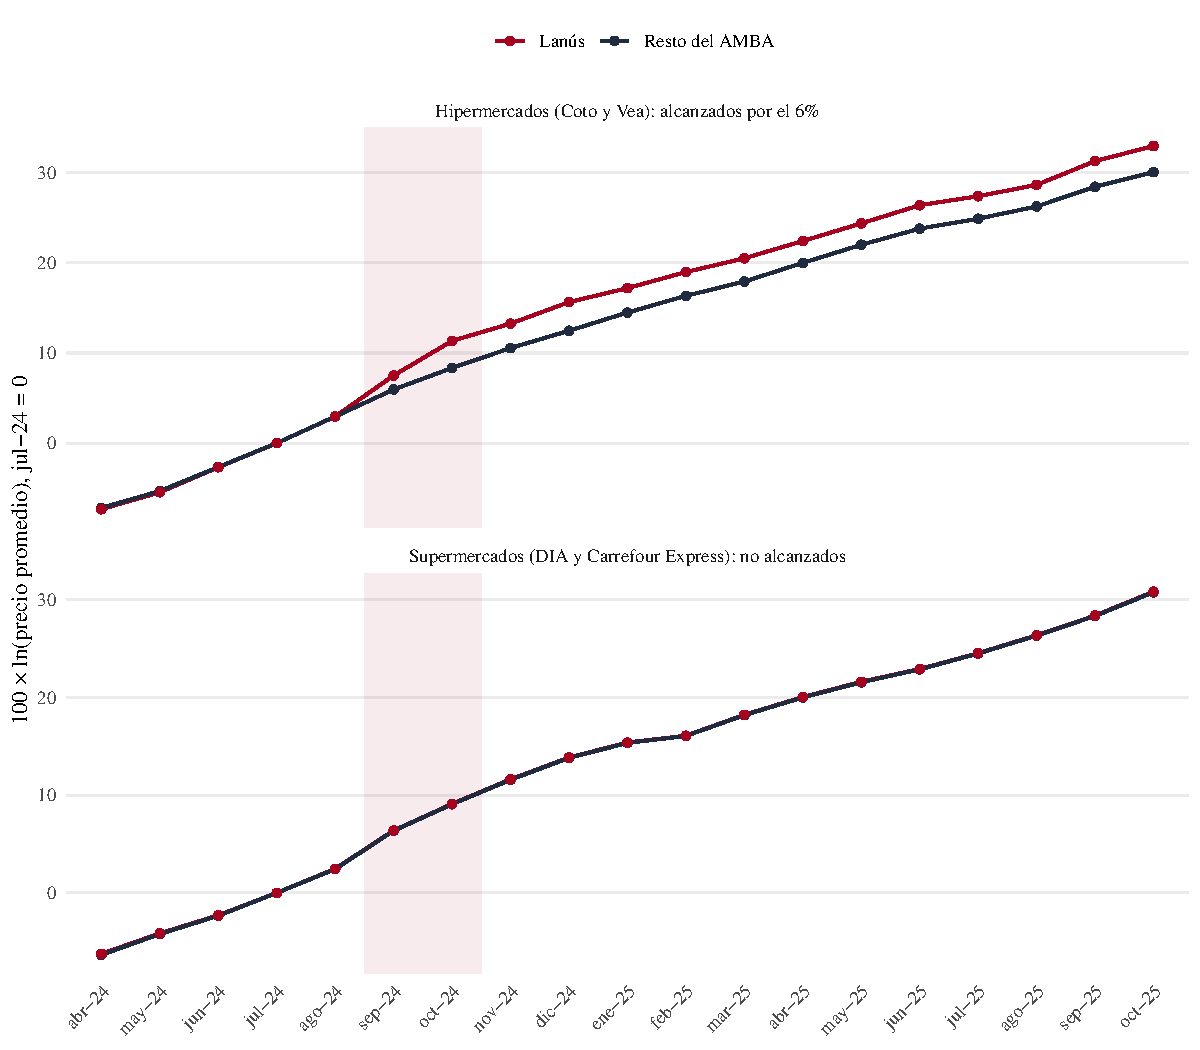
\includegraphics[width=0.65\linewidth]{figuras/tendencias.pdf}
  \nota{100 \(\times\) logaritmo del precio promedio de la canasta de cada formato, julio de 2024 = 0. Mismo producto y mismo
  formato de local; para el resto del AMBA se promedia entre partidos y los formatos tienen igual peso. La franja sombreada
  marca septiembre y octubre de 2024.}
\end{figure}

\begin{table}[htbp]
  \caption{Efecto del aumento de la tasa sobre los precios de los hipermercados de Lanús}
  \label{tab:did}
  \centering\small
  \begin{tabular}{lcccc}
\toprule
 & (1) & (2) & (3) & (4) \\
 & Hipermercados & Hipermercados & Coto & Vea \\
\midrule
Lanús $\times$ Post & 3,52 & 3,22 & 3,42 & 2,30 \\
 & (0,09) & (0,05) & (0,06) & (0,10) \\
p-valor de permutación & & 0,048 & 0,048 & 0,125 \\
\midrule
EF unidad & Sí & Sí & Sí & Sí \\
EF mes & Sí & & & \\
EF producto$\times$formato$\times$mes & & Sí & Sí & Sí \\
Partidos & 21 & 21 & 21 & 8 \\
Observaciones & 980.305 & 980.305 & 898.569 & 81.736 \\
Traslado (\%) & & 83 & 89 & 59 \\
\bottomrule
\end{tabular}

  \nota{estimación de la ecuación~\eqref{eq:2}. Variable dependiente: 100 \(\times\) ln(precio). Errores estándar agrupados
  por producto entre paréntesis. El p-valor de permutación se calcula según la sección~5. Ventana: abril de 2024 a octubre
  de 2025, sin agosto ni septiembre de 2024. Traslado = efecto estimado / 3,86. EF: efectos fijos.}
\end{table}

\begin{table}[htbp]
  \caption{Estudio de eventos: hipermercados de Lanús}
  \label{tab:es}
  \centering\small
  \begin{tabular}{lcc|lcc}
\toprule
Mes & $\delta_k$ & (e.e.) & Mes & $\delta_k$ & (e.e.) \\
\midrule
abr-24 & -0,10 & (0,03) & feb-25 & 3,24 & (0,09) \\
may-24 & -0,09 & (0,02) & mar-25 & 3,14 & (0,07) \\
jun-24 & 0,02 & (0,02) & abr-25 & 3,14 & (0,07) \\
jul-24 & 0,00 & ref. & may-25 & 3,20 & (0,08) \\
ago-24 & 0,04 & (0,02) & jun-25 & 3,26 & (0,08) \\
sep-24 & 1,49 & (0,05) & jul-25 & 3,14 & (0,07) \\
oct-24 & 3,03 & (0,05) & ago-25 & 3,00 & (0,06) \\
nov-24 & 3,17 & (0,07) & sep-25 & 3,13 & (0,06) \\
dic-24 & 3,35 & (0,07) & oct-25 & 3,19 & (0,06) \\
ene-25 & 3,24 & (0,08) &  & &  \\
\bottomrule
\end{tabular}

  \nota{estimación de la ecuación~\eqref{eq:6}. Coeficientes en puntos porcentuales; referencia: julio de 2024. Errores
  estándar agrupados por producto entre paréntesis.}
\end{table}

\begin{figure}[htbp]
  \caption{Estudio de eventos: hipermercados de Lanús}
  \label{fig:es}
  \centering
  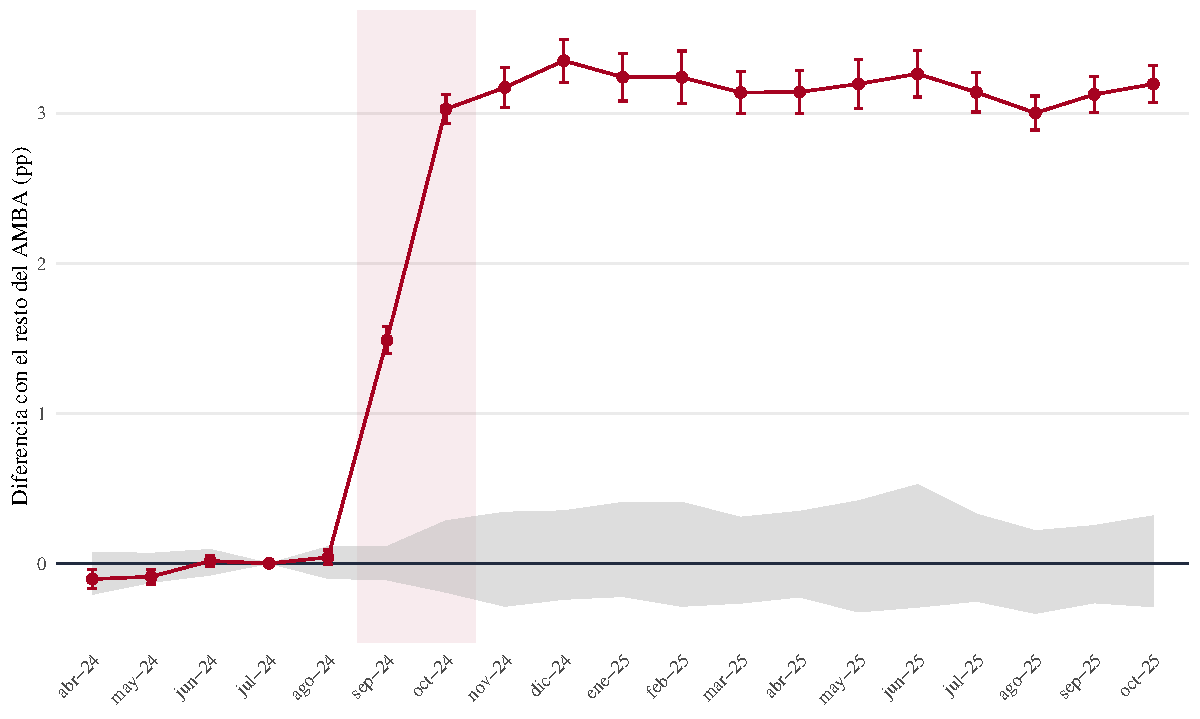
\includegraphics[width=0.85\linewidth]{figuras/event_study.pdf}
  \nota{coeficientes de la ecuación~\eqref{eq:6} con intervalos de confianza del 95\% (errores agrupados por producto);
  referencia: julio de 2024. La franja gris muestra el rango de coeficientes que se obtiene al asignar el tratamiento a cada
  uno de los demás partidos. La franja sombreada marca septiembre y octubre de 2024.}
\end{figure}

\begin{figure}[htbp]
  \caption{Inferencia por permutación: efecto estimado al asignar el tratamiento a cada partido}
  \label{fig:perm}
  \centering
  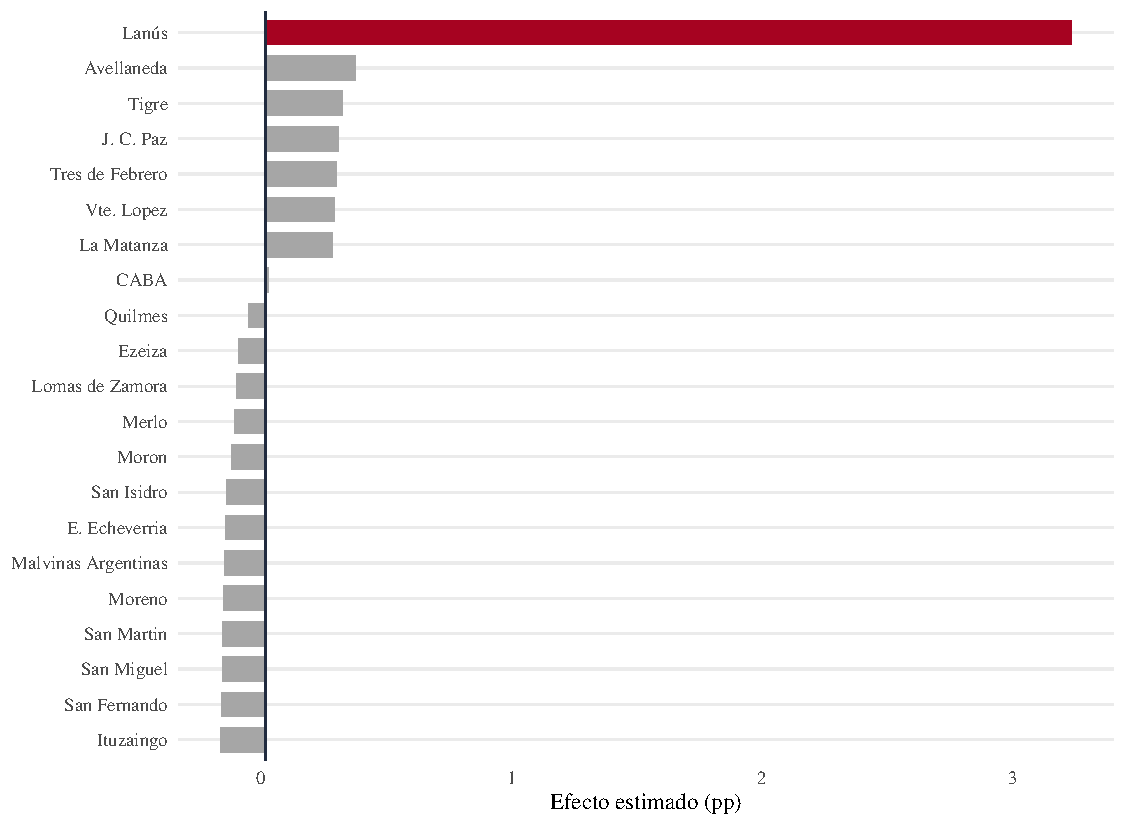
\includegraphics[width=0.68\linewidth]{figuras/permutacion.pdf}
  \nota{hipermercados (Coto y Vea). Cada barra es el coeficiente de la ecuación~\eqref{eq:2} estimado asignando el
  tratamiento al partido indicado, sin Lanús en la muestra de control. P-valor de permutación de Lanús: 0,048.}
\end{figure}

\begin{table}[htbp]
  \caption{Prueba placebo: supermercados de Lanús (no alcanzados por el aumento)}
  \label{tab:placebo}
  \centering\small
  \begin{tabular}{lccc}
\toprule
Supermercados & $\hat\delta$ (pp) & (e.e.) & p-valor de permutación \\
\midrule
Total (DIA y Carrefour Express) & -0,02 & (0,01) & 0,667 \\
DIA & -0,02 & (0,01) & 0,625 \\
Carrefour Express & -0,02 & (0,02) & 0,818 \\
\bottomrule
\end{tabular}

  \nota{estimación de la ecuación~\eqref{eq:2} para los supermercados de Lanús (DIA y Carrefour Express), comparados con
  los mismos formatos en el resto del AMBA. Errores estándar agrupados por producto entre paréntesis.}
\end{table}

\begin{figure}[htbp]
  \caption{Prueba placebo: estudio de eventos para los supermercados de Lanús}
  \label{fig:es_placebo}
  \centering
  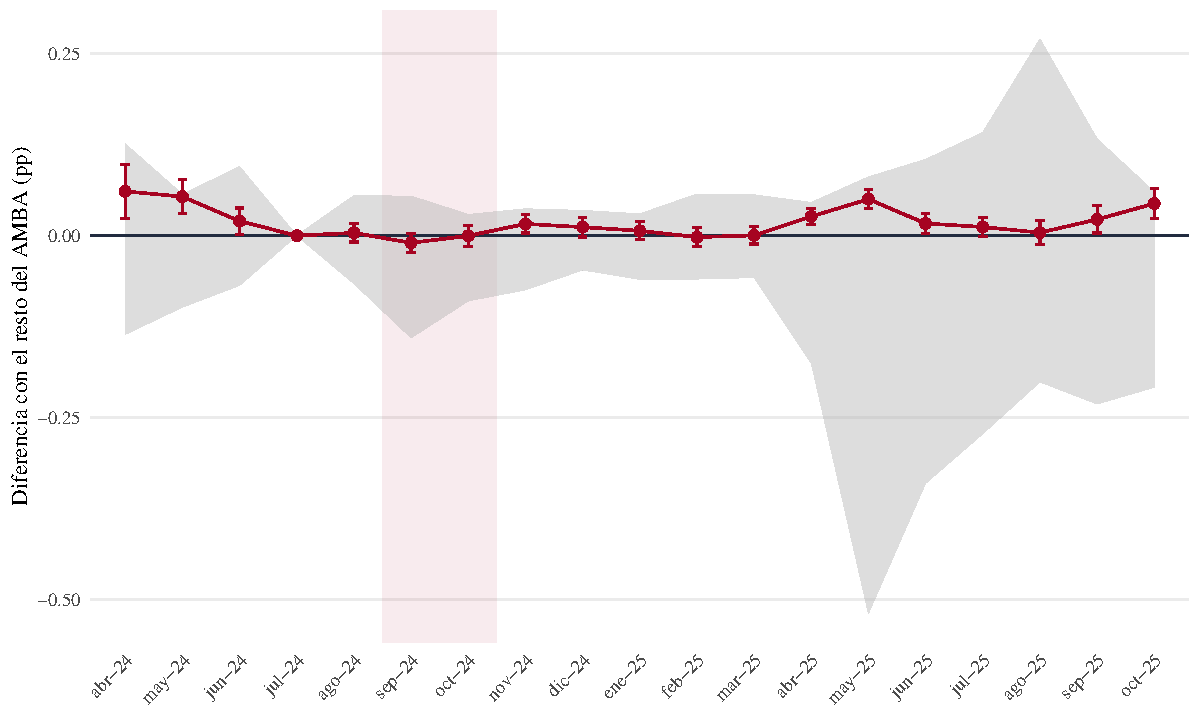
\includegraphics[width=0.85\linewidth]{figuras/event_study_placebo.pdf}
  \nota{coeficientes de la ecuación~\eqref{eq:6} estimada para los supermercados (DIA y Carrefour Express), con intervalos
  de confianza del 95\% (errores agrupados por producto); referencia: julio de 2024. La franja gris muestra el rango de
  coeficientes de los demás partidos.}
\end{figure}


\end{document}
